\chapter{Auswertung der Messdaten}
    \section{Kalibrierung}
        Bevor man die Werte auslesen kann muss eine Kalibrierung gemacht werden. Diese wurde von Herrn Dörr durchgeführt. In der Datei \texttt{Kalibriermessung\_3.txt} 
        befinden sich die Signalausgabe des Beschleunigungssensors während der Kalibrierung.
        Diese Werte werden in der Grafik~\ref{kaligraf} mit Hilfe von SciDAVis veranschaulicht.\\
        \begin{figure}[ht!]
            \centering
            \includegraphics[width=\linewidth]{images/kalibrierung.png}
            \caption{grafische Darstellung der Kalibrierwerte}
            \label{kaligraf}
        \end{figure}
        
        \subsection{Bestimmung des Kalibrierfaktors}
            Mit dem Courser-Tool werden die Werte \(ADC_{z1}\) und \(ADC_{z2}\) ausgelesen. 
            \begin{table}[!ht]
                \centering
                \caption{Messwerte \(ADC_{z1}\) und \(ADC_{z2}\) der Kalibrierung}
                \begin{tabular}{|c|c|}
                    \hline
                    \(ADC_{z1}\) & \(ADC_{z2}\)\\ \hline 
                    1292 & 844 \\ \hline
                \end{tabular}
                \label{kali}
            \end{table}
            Setzt man nun die Werte in die Gleichung 3 aus dem Aufgabenblatt ein, so ergibt sich folgende Rechnung.
            \begin{align*}
                k_z&=\frac{a_{z1}-a_{z2}}{ADC_{z1}-ADC_{z2}}\\
                &=\frac{2\cdot \SI{9.81}{\meter\per\square\second}}{1292-844}\\
                &=\SI{0,044}{\meter\per\square\second}
            \end{align*}
        \subsection{Bestimmung des Offset's $ADC_{z0}$}
            Um Offset \(ADC_{z0}\) bestimmen zu können werden die Werte aus der Tabelle~\ref{kali} in die Gleichung 4 aus dem Aufgabenblatt eingesetzt. 
            \begin{align*}
                ADC_{z0}&=\frac{ADC_{z1}+ADC_{z2}}{2}\\
                &=\frac{1292+844}{2}\\
                &=1068 
            \end{align*}
        \subsection{Vergleich des \(k_z\) Wert mit der Empfindlichkeit des Datenblatts}
            Die Empfindlichkeit, die im Datenblatt angegeben wird, hat mit dem \(k_z\) Wert nichts direkt zu tun. Die Empfindlichkeit bezieht sich auf die Messgenauigkeit des Sensors. 
            Der \(k_z\) Wert ist an die örtliche Gegebenheit ausgelegt. Dieser Faktor beschreibt das Verhältnis der digitalen Ausgangsgröße zu der physikalischen Größe.
    \section{Beschreibung des verwendeten Blockdiagramms} 
        Das gesamte Blockdiagram wird von einer While-Schleife umschlossen. Diese wird nach einer Ausführung für \SI{1000}{\milli\second} angehalten. 
        Ebenso befindet sich dort die Abbruchfunktion über den Stop-Button.\par
        Die Datei, mit den Messdaten, wird über ein \textbf{Path-Module} eingelesen und wird an das Modul \textbf{Tabelle auslesen} weiter gereicht. Darauf folgt die lesung der Spalten. Mit den Konstanten \textbf{0} und \textbf{3} geben wir an, dass wir aus den Messdaten die Spalte 0, mit der gemessenen Zeit und Spalte 3 mit dem Ausgangssignal in z-Richtung.
        Aus dem Datenstrom der Spalte ein lässt sich die maximale Zeilenanzahl auslese und wird an eine numerische Frontpanel-Ausgaben weiter geschleift.
        Dieser Datenstrom wird auch noch für die jeweilige Grafen als X-Wert eingebunden. \par
        Der Datenstrom der aus Aus der Spalte 3 ausgelesen wird, wird zunächst an eine Savitzky-Golay-Filter weitergeleitet mit eine Angabe von 20 Seitenpunkte.
        Im Anschluss wird der \textbf{Offset a} von dem Datenstrom subtrahiert und der \(k_z\)-Wert multipliziert. Das Ergebnis geht nun weiter an den ersten Graf und wird hier als Y-Wert eingebunden. 
        Zusätzlich wird von diesem Wert der \textbf{Offset v} subtrahiert und im Anschluss in ein Integrations Modul weitergeleitet. Für d(t) wird der Wert 0,005 dem Modul angegeben. Das Ergebnis aus diesem Mudol wird in den Graf für die Geschwindigkeit als Y-Wert eingebunden und gleichzeitig nochmals auf die selbe Weise integriert.
        Nach der zweiten Integration wird auch dieser Wert in eine Graf als Y-Wert eingebunden. Dieser Graf beschreibt die zurückgelegte Strecke.
        \begin{figure}[ht!]
            \centering
            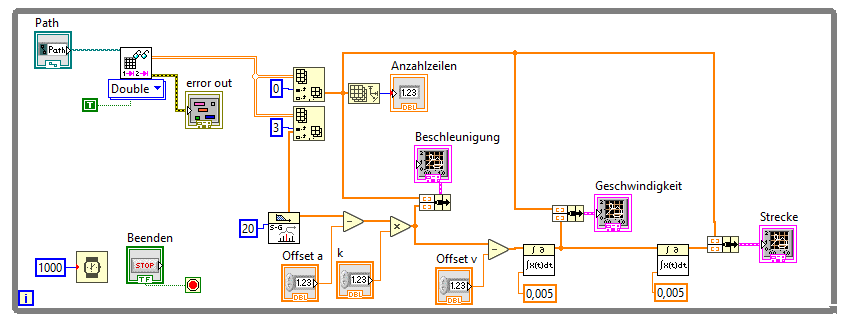
\includegraphics[width=\linewidth]{images/blockdiagramm.PNG}
            \caption{Blockdiagramm aus LabVIEW}
            \label{block}
        \end{figure}
    \section{Front Panel}
        \begin{figure}[ht!]
            \centering
            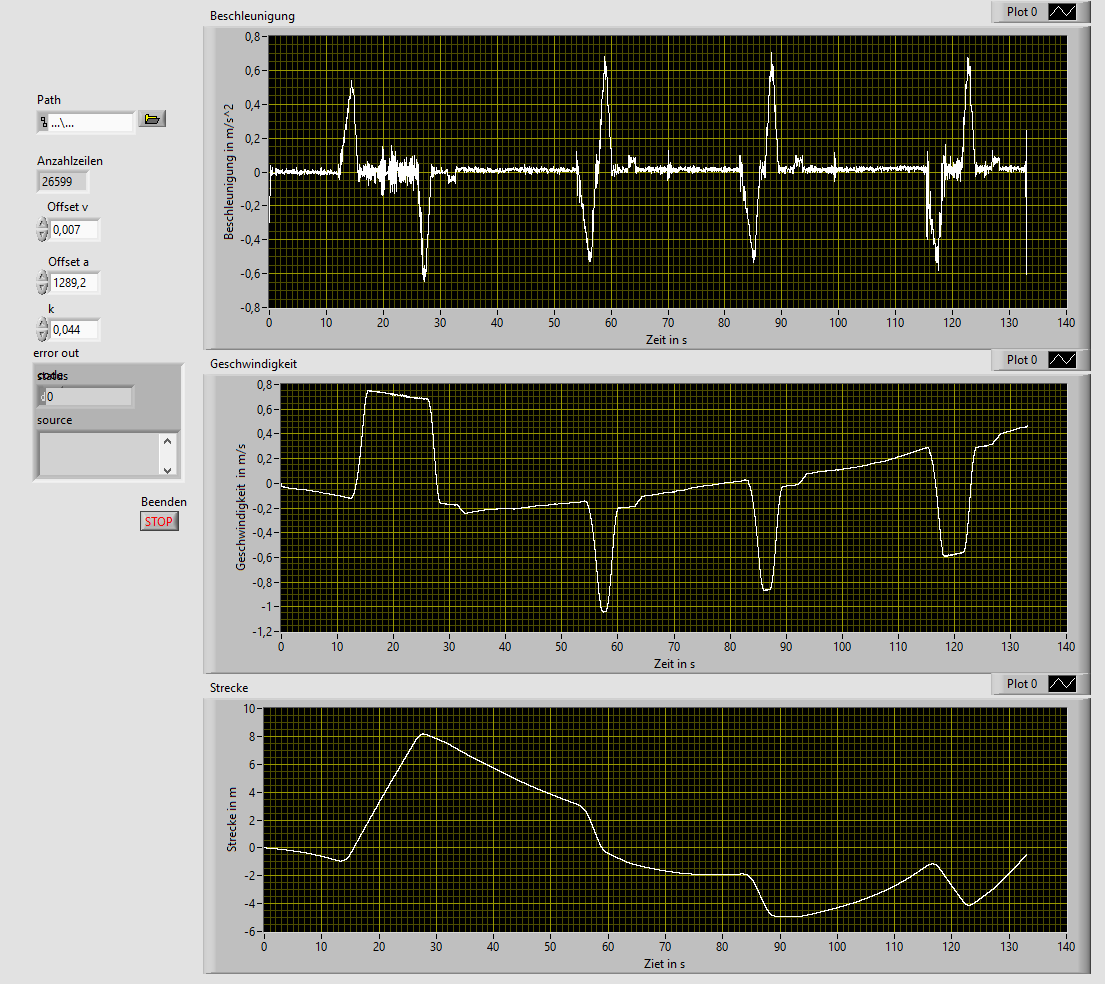
\includegraphics[width=\linewidth]{images/vi.PNG}
            \caption{VI was in LabVIEW erstellt wurde}
            \label{vi}
        \end{figure}
        
    \section{\textit{a(t)-, v(t)-, s(t)-Diagramm}}
        
        \subsection{Ermittlung des Offset's \textit{a} und \textit{v}}
            Für die Ermittlung von \textbf{Offset a} haben wir den ersten Wert aus der vierten Spalte der Messdaten abgelesen. Hier stand ein Wert von 1289. Durch ausprobieren kommen wir auf einen Wert von 1289,2  \par
            Die Ermittlung des \textbf{Offset v} ergab durch ausprobieren einen Wert von 0,007. Damit ist der Endpunkt der Strecke wieder auf der Nulllinie.
        \subsection{Ermittlung von $a_{max}$, $v_{max}$ und $s_{ges}$}
            Bei der Ermittlung der Werte für $a_{max}$, $v_{max}$ und $s_{ges}$ haben wir die jeweilige Werte aus den Abbildungen abgelesen. 
            Hierbei haben wir folgende Werte feststellen können.\par
            Für die maximale Beschleunigung haben wir einen Wert von ca. \SI{0,7}{\meter\per\square\second} ablesen können.\\
            Für die maximale Geschwindigkeit haben wir einen Wert von ca. \SI{0,9}{\meter\per\second} ermitteln können.
            Für die gesamte Strecke haben wir einen Wert von ca. \SI{9}{\meter} feststellen können.
            \begin{figure}[ht!]
                \centering
                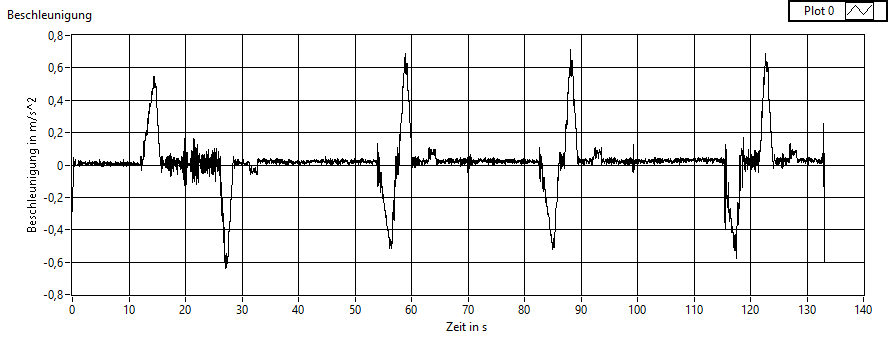
\includegraphics[width=\linewidth]{images/beschleunigung.png}
                \caption{Messwerte umgerechnet in Beschleunigung}
            \end{figure}
            \begin{figure}[ht!]
                \centering
                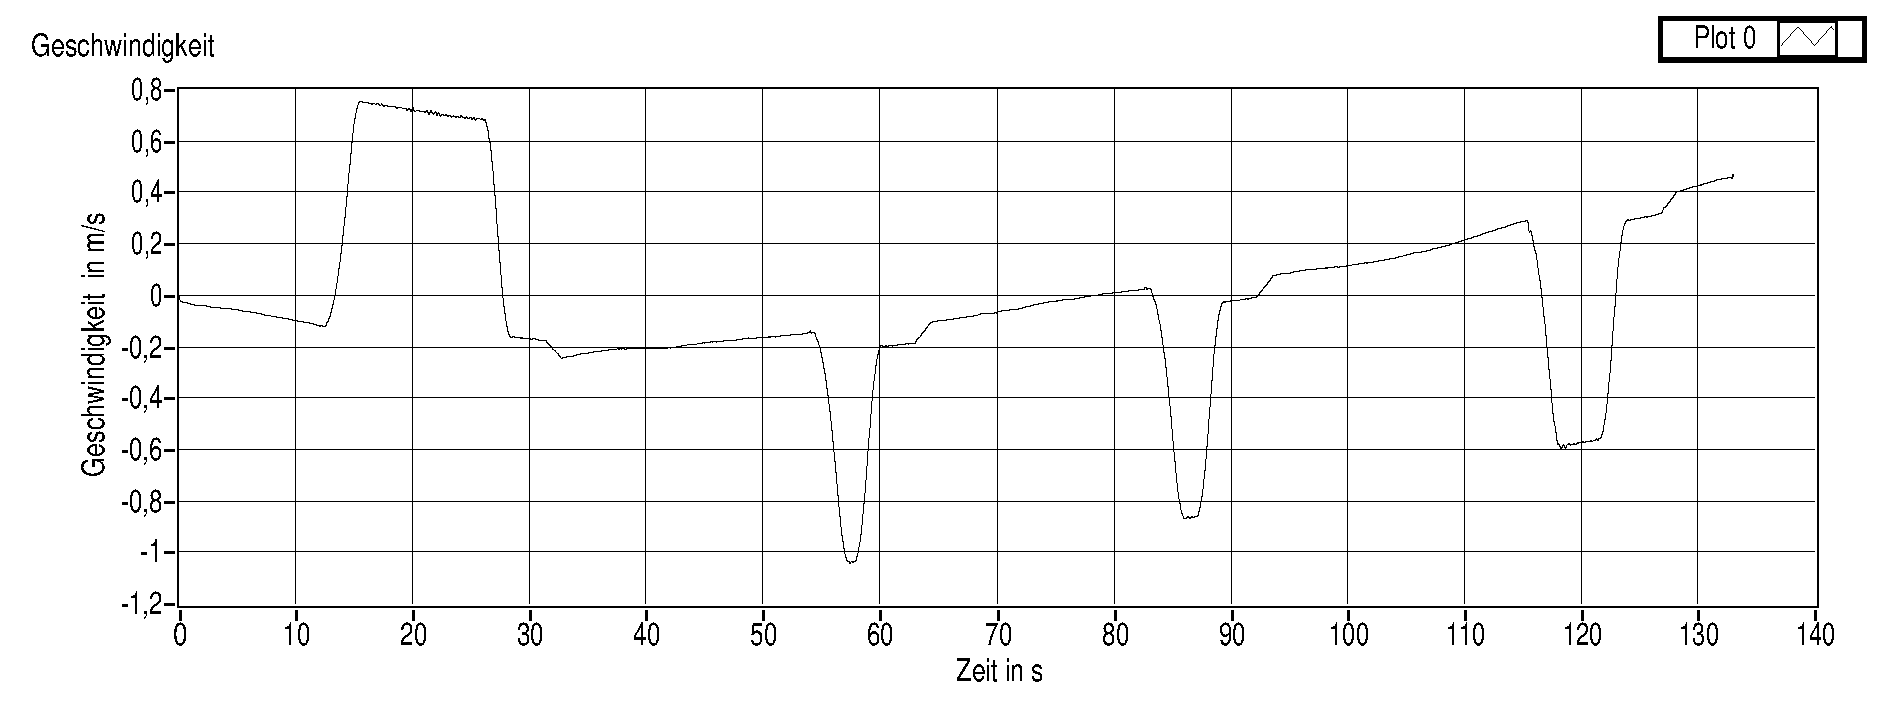
\includegraphics[width=\linewidth]{images/geschwindigkeit.eps}
                \caption{Geschwindigkeit aus den Werten der Beschleunigung integriert}
            \end{figure}
            \begin{figure}[ht!]
                \centering
                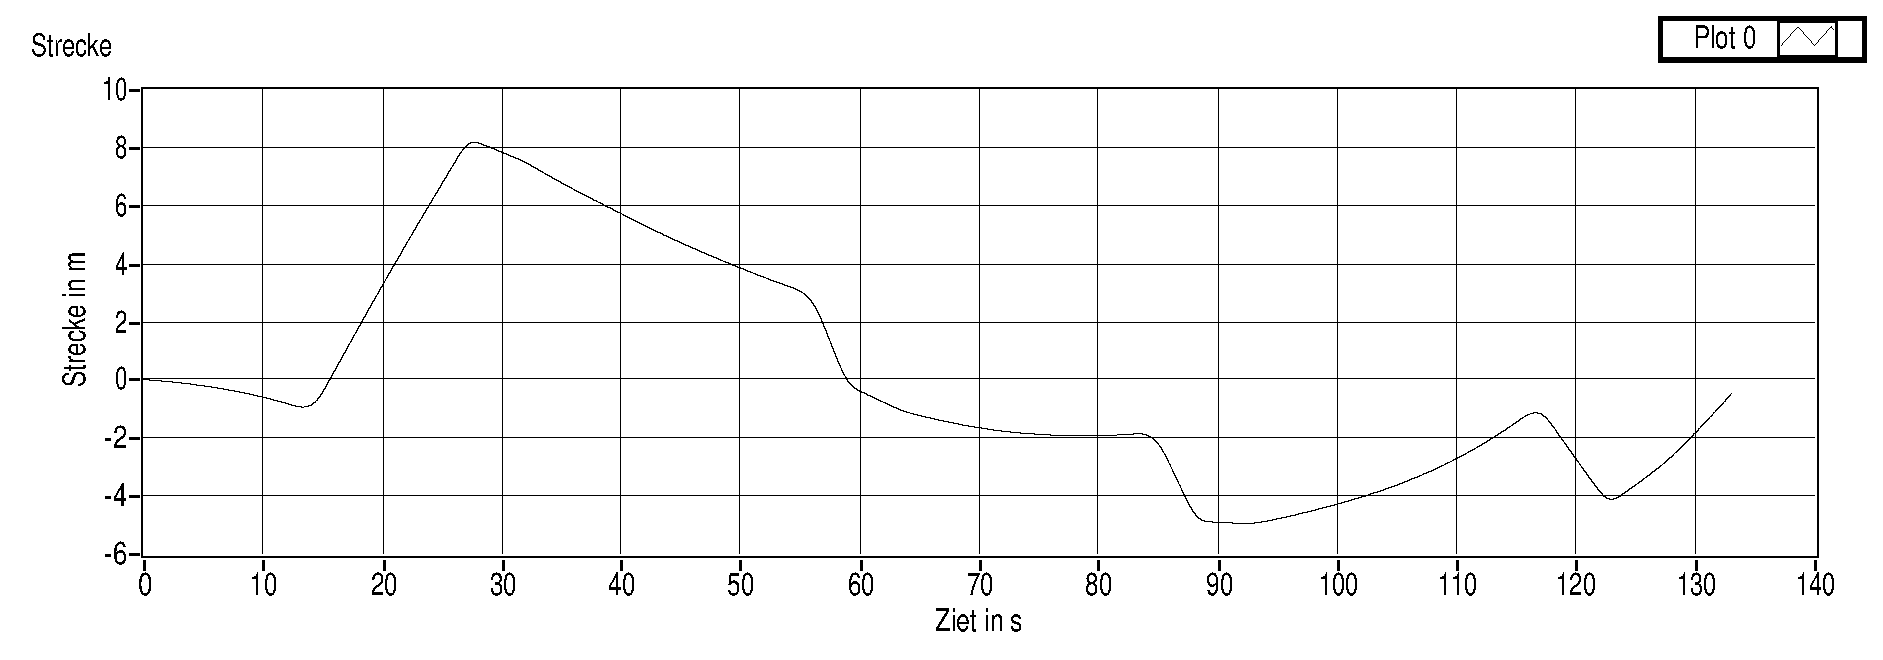
\includegraphics[width=\linewidth]{images/strecke.eps}
                \caption{Zurückgelegte Strecke aus den Werten der Geschwindigkeit integriert}
            \end{figure}
    \section{Messauflösung $a_{LSB}$}    
        Die Ermittlung des \(a_{LSB}\) haben wir mit Hilfe des \textbf{Offset a} und dem Wert der Erdbeschleunigung versucht zu berechnen.
        Hierbei sind wir wie folgt vorgegangen.
        \begin{align*}
            a_{LSB}&= \frac{g}{\textmd{Offset a}}\\
            &=\frac{\SI{9,81}{\meter\per\square\second}}{1298}\\
            &=\SI{0,008}{\meter\per\square\second}
        \end{align*}